% !TeX root = main.tex

\setlength{\abovedisplayskip}{7pt}
\setlength{\belowdisplayskip}{7pt}
\setlength{\abovedisplayshortskip}{4pt}
\setlength{\belowdisplayshortskip}{4pt}

\makeatletter
\newenvironment{reportfigure}{%
  \par\addvspace{6pt}\noindent
  \begin{minipage}{\textwidth}\def\@captype{figure}\centering
}{\end{minipage}\par\vspace{4pt}}
\makeatother

\tableofcontents
\newpage

\section{Система 1}

Рассмотрим систему
\begin{equation}
  \begin{cases}
    \dot x_1=x_2+\sin x_1,\\
    \dot x_2=\theta_1x_1^2+(2+\theta_2)u
  \end{cases}
  \qquad |\theta_1|\le1,\quad |\theta_2|\le1
\end{equation}
Выберем поверхность скольжения
\begin{equation}
  s=x_1+x_2+\sin x_1
\end{equation}
Тогда $\dot x_1=-x_1+s$, а на $s=0$ получаем
$\dot x_1=-x_1$. Производная $s$ равна
\begin{equation}
  \dot s=(1+\cos x_1)(x_2+\sin x_1)+\theta_1x_1^2+(2+\theta_2)u
\end{equation}
Поскольку $2+\theta_2\ge1$, выбираем
\begin{equation}
  \varrho(\bm x)=\left|(1+\cos x_1)(x_2+\sin x_1)\right|+x_1^2,
  \qquad \beta(\bm x)=\varrho(\bm x)+1
\end{equation}
Оба регулятора ниже используют только измеряемое состояние.

\subsection{Разрывный регулятор}

Закон управления имеет вид
\begin{equation}
  u=-\beta(\bm x)\sgn s
\end{equation}
Для $V=s^2/2$ при $s\ne0$ получаем
\begin{equation}
  \dot V=s\dot s\le-(2+\theta_2)|s|\le-|s|
\end{equation}
Поэтому поверхность достигается за $t_*\le|s(0)|$.
Разрывный закон понимается в смысле Филиппова. После достижения
поверхности $x_1(t)\to0$, $x_2=-x_1-\sin x_1\to0$.
До достижения $s$ ограничен, а $\dot x_1=-x_1+s$ обеспечивает
ограниченность состояний. Следовательно, начало координат глобально
асимптотически устойчиво.

\subsection{Непрерывный регулятор}

Заменим знак насыщением:
\begin{equation}
  u=-\beta(\bm x)\operatorname{sat}\frac{s}{\varepsilon},
  \qquad 0<\varepsilon\le\frac14,
  \qquad
  \operatorname{sat}y=
  \begin{cases}
    y,& |y|\le1,\\
    \sgn y,& |y|>1
  \end{cases}
\end{equation}
При $|s|\ge\varepsilon$ сохраняется $\dot V\le-|s|$.
Полоса $|s|\le\varepsilon$ инвариантна и достигается за
$t_\varepsilon\le\max\{|s(0)|-\varepsilon,0\}$.
Внутри полосы для $V_c=(x_1^2+s^2)/2$ имеем
\begin{equation}
  \begin{aligned}
    \dot V_c={}&-x_1^2-\cos x_1\,x_1s+(1+\cos x_1)s^2
      +\theta_1x_1^2s-\frac{(2+\theta_2)\beta}{\varepsilon}s^2\\
    \le{}&-\frac{x_1^2}{2}
      +\left(3+x_1^2-\frac{\beta}{\varepsilon}\right)s^2\\
    \le{}&-\frac{x_1^2}{2}-(1+3x_1^2)s^2\le-V_c
  \end{aligned}
\end{equation}
Здесь использованы $|x_1s|+x_1^2|s|\le x_1^2/2+(1+x_1^2)s^2$
и $\beta\ge1+x_1^2$. Следовательно, непрерывный регулятор также
обеспечивает глобальную асимптотическую устойчивость начала координат.

\subsection{Моделирование}

Примем $\theta_1=1$, $\theta_2=-1$, $\bm x(0)=(1,0)^T$
и $\varepsilon=0{,}1$. Моделирование выполнено методом Рунге-Кутты
четвёртого порядка с шагом $0{,}001$ на интервале $t\in[0,12]$.
Для разрывного закона определялся момент достижения $s=0$,
после которого использовалась идеальная скользящая динамика
и эквивалентное управление по модели.

\begin{reportfigure}
  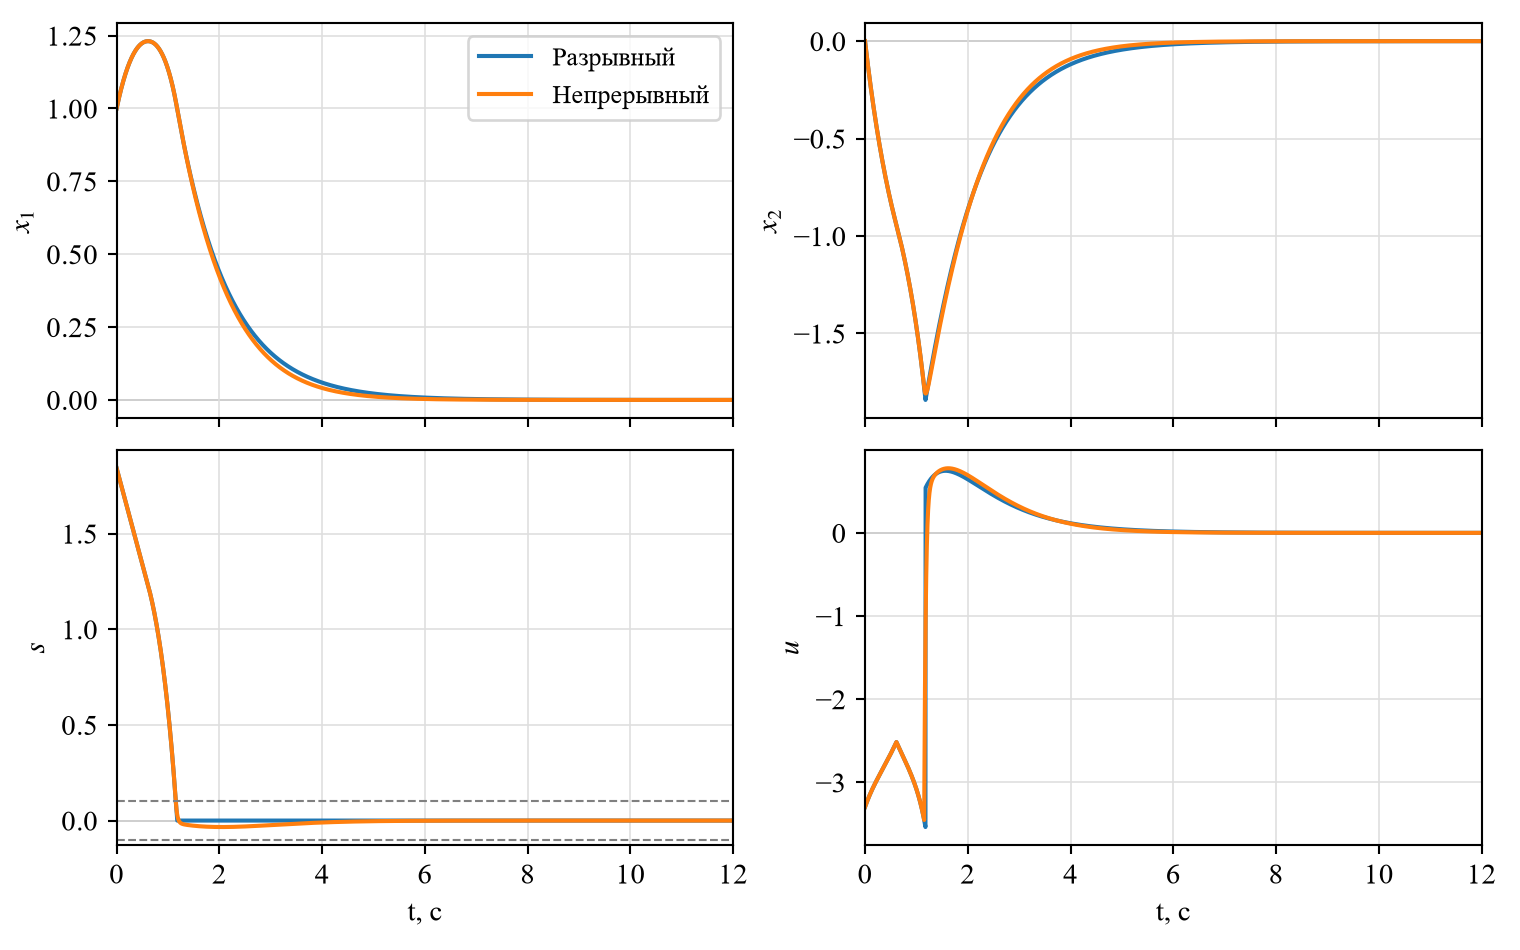
\includegraphics[width=0.96\textwidth]{task1_comparison.png}
  \caption{Состояния, поверхность скольжения и управление системы 1}
\end{reportfigure}

Оба регулятора обеспечивают сходимость состояний к нулю.
При разрывном законе поверхность достигается при $t_*\approx1{,}177$;
при непрерывном законе полоса $|s|\le0{,}1$ достигается
при $t\approx1{,}152$. Далее $s$ также стремится к нулю.

\section{Система 2}

Исходная система имеет вид
\begin{equation}
  \begin{cases}
    \dot x_1=x_2+a_1x_1\sin x_1,\\
    \dot x_2=a_2x_1x_2+3u
  \end{cases}
  \qquad a_1,a_2\in[0,2]
\end{equation}
Выберем $s=3x_1+x_2$. На поверхности $s=0$ получаем
\begin{equation}
  \dot x_1=(-3+a_1\sin x_1)x_1,\qquad
  x_1\dot x_1\le-x_1^2
\end{equation}
Поэтому динамика на поверхности глобально асимптотически устойчива.
Поскольку
\begin{equation}
  \dot s=3x_2+3a_1x_1\sin x_1+a_2x_1x_2+3u,
\end{equation}
можно принять
\begin{equation}
  \varrho(\bm x)=|x_2|+2|x_1\sin x_1|+\frac23|x_1x_2|,
  \qquad \beta=\varrho+1,\qquad u=-\beta\sgn s
\end{equation}
Для $V=s^2/2$ имеем $\dot V\le-3|s|$,
следовательно, $t_*\le|s(0)|/3$.
До достижения поверхности $s$ ограничен и
$\frac{d}{dt}|x_1|\le-|x_1|+|s|$ почти всюду,
поэтому состояния остаются ограниченными.
После достижения $|x_1(t)|\le|x_1(t_*)|e^{-(t-t_*)}$ и $x_2=-3x_1$.
Начало координат глобально асимптотически устойчиво.

Моделирование проведено при $a_1=a_2=2$, $\bm x(0)=(1{,}5;0)^T$,
$t\in[0,12]$ с тем же шагом и обнаружением идеального скольжения.

\begin{reportfigure}
  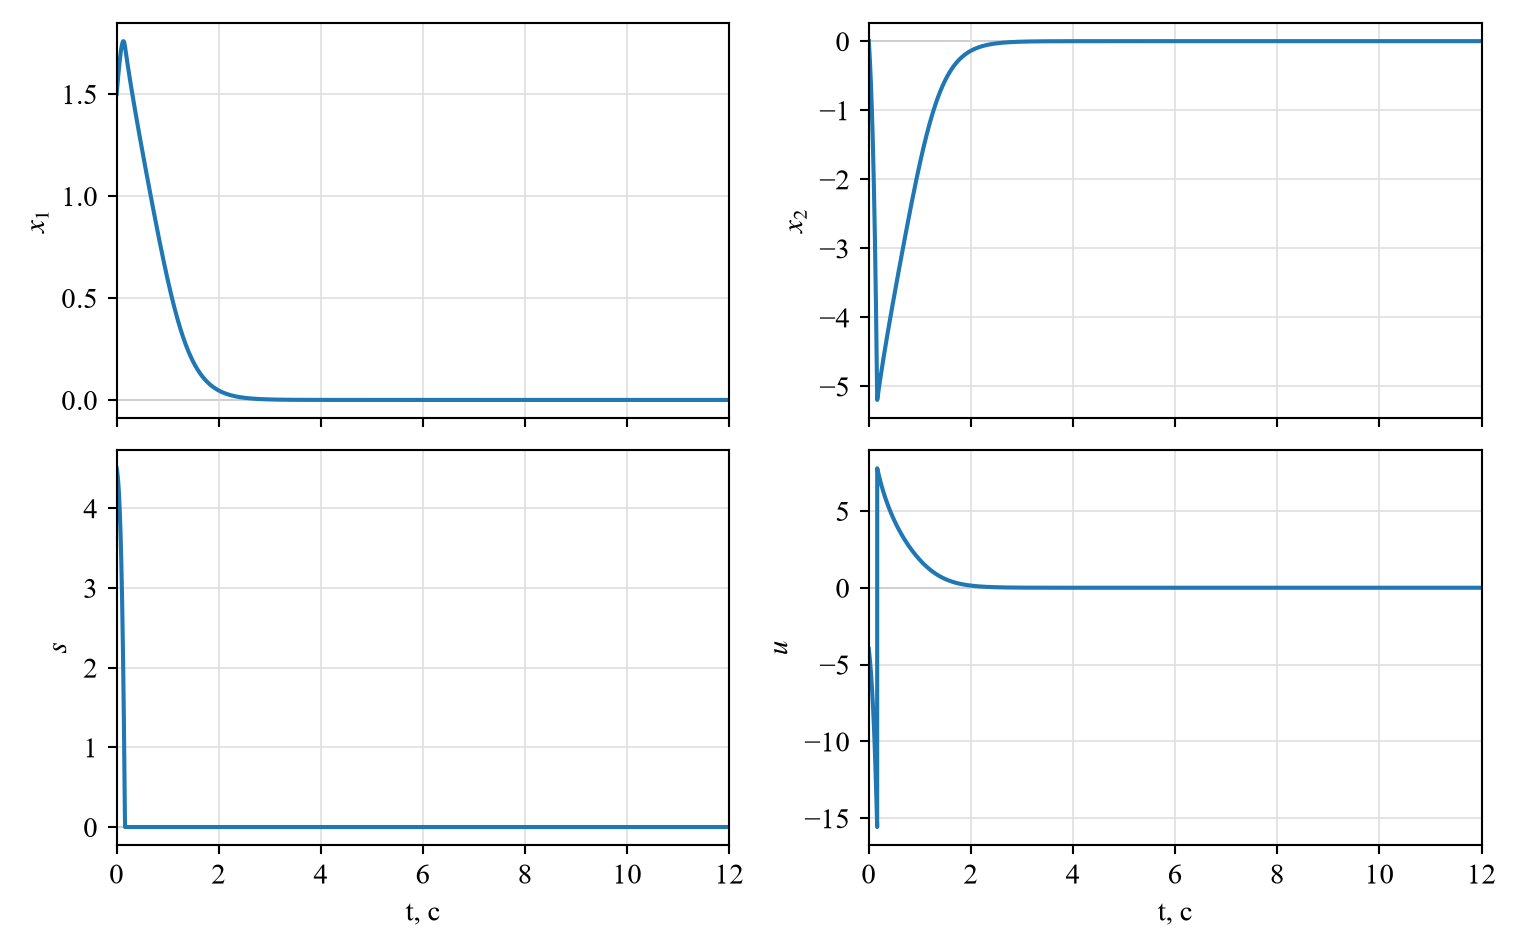
\includegraphics[width=0.96\textwidth]{task2_sliding.png}
  \caption{Состояния, поверхность скольжения и управление системы 2}
\end{reportfigure}

Поверхность достигается при $t_*\approx0{,}163$,
после чего состояния стремятся к нулю.

\section{Непрерывное управление маятником}

Уравнение движения имеет вид
\begin{equation}
  ml\ddot\theta+mg\sin\theta+kl\dot\theta
  =\frac{T}{l}+mh(t)\cos\theta
\end{equation}
Заданы $0{,}8\le l\le1$, $0{,}5\le m\le1$,
$0{,}1\le k\le0{,}2$, $|h(t)|\le0{,}5$, $g=9{,}81$.
Положим $x_1=\theta$, $x_2=\dot\theta$, $s=x_1+x_2$. Тогда
\begin{equation}
  ml^2\dot s=l^2(m-k)x_2-mgl\sin x_1+mlh(t)\cos x_1+T
\end{equation}
Неопределённая часть по модулю не превосходит
\begin{equation}
  \varrho(\bm x)=0{,}9|x_2|+9{,}81|\sin x_1|+0{,}5|\cos x_1|
\end{equation}
Искомый непрерывный регулятор:
\begin{equation}
  T=-\bigl(\varrho(\bm x)+1\bigr)
       \operatorname{sat}\frac{s}{\varepsilon},\qquad \varepsilon>0
\end{equation}
При $|s|\ge\varepsilon$ функция $V=s^2/2$ удовлетворяет оценке
\begin{equation}
  \dot V\le-\frac{|s|}{ml^2}\le-|s|
\end{equation}
Поэтому полоса $|s|\le\varepsilon$ инвариантна и достигается за
$t_\varepsilon\le\max\{|s(0)|-\varepsilon,0\}$.
Из $\dot\theta=-\theta+s$ после входа в полосу следует
\begin{equation}
  \begin{gathered}
    |\theta(t)|\le e^{-(t-t_\varepsilon)}|\theta(t_\varepsilon)|
       +\varepsilon\bigl(1-e^{-(t-t_\varepsilon)}\bigr),\\
    \limsup_{t\to\infty}|\theta(t)|\le\varepsilon,\qquad
    \limsup_{t\to\infty}|\dot\theta(t)|\le2\varepsilon
  \end{gathered}
\end{equation}
До входа $s$ ограничен, поэтому состояния также ограничены.
Получена глобальная практическая стабилизация: при
$\varepsilon=0{,}05$ предельные оценки равны $0{,}05$ рад
и $0{,}1$ рад/с. Точное удержание нуля при произвольном неизвестном
$h(t)$ потребовало бы $T(0,0)=-mlh(t)$.
